\documentclass{report}
\usepackage{tikz, calc}
\usepackage{comment}
\usepackage{xifthen}
\usepackage{amsmath}
\usepackage{lscape}

\usetikzlibrary{positioning}
\definecolor{myyellow}{RGB}{255,250,205}

\begin{document}

\begin{landscape} %horizontal page 
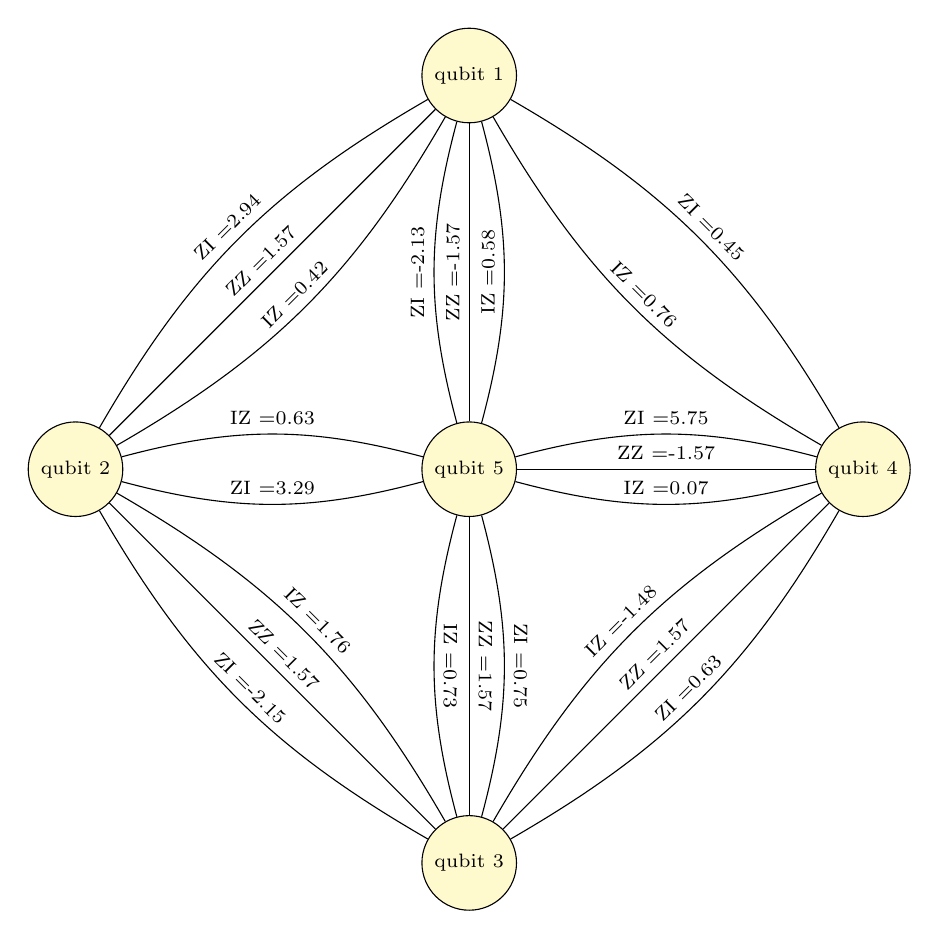
\begin{tikzpicture}



\foreach \a in {1,2,...,4}{
	\draw (\a*360/4: 5cm) node [circle, draw, fill = myyellow, align=center] (\a) {\scriptsize qubit \a};
};

\draw (0:0) node [circle, draw, fill = myyellow, align=center] (5) {\scriptsize qubit 5};




%----------INNER LINKS-------------%
\draw[-]
(2) to [bend right = 0] node[sloped, above] {\scriptsize ZZ =1.57} (1);
\draw[-]
(2) to [bend right = 15] node[sloped, above] {\scriptsize IZ =0.42} (1);
\draw[-]
(2) to [bend right = -15] node[sloped, above] {\scriptsize ZI =2.94} (1);
\draw[-]
(5) to [bend right = 0] node[sloped, above] {\scriptsize ZZ =-1.57} (1);
\draw[-]
(5) to [bend right = 15] node[sloped, above] {\scriptsize IZ =0.58} (1);
\draw[-]
(5) to [bend right = -15] node[sloped, above] {\scriptsize ZI =-2.13} (1);
\draw[-]
(3) to [bend right = 0] node[sloped, above] {\scriptsize ZZ =1.57} (2);
\draw[-]
(3) to [bend right = 15] node[sloped, above] {\scriptsize IZ =1.76} (2);
\draw[-]
(3) to [bend right = -15] node[sloped, above] {\scriptsize ZI =-2.15} (2);
\draw[-]
(5) to [bend right = 15] node[sloped, above] {\scriptsize IZ =0.63} (2);
\draw[-]
(5) to [bend right = -15] node[sloped, above] {\scriptsize ZI =3.29} (2);
\draw[-]
(4) to [bend right = 0] node[sloped, above] {\scriptsize ZZ =1.57} (3);
\draw[-]
(4) to [bend right = 15] node[sloped, above] {\scriptsize IZ =-1.48} (3);
\draw[-]
(4) to [bend right = -15] node[sloped, above] {\scriptsize ZI =0.63} (3);
\draw[-]
(5) to [bend right = 0] node[sloped, above] {\scriptsize ZZ =1.57} (3);
\draw[-]
(5) to [bend right = 15] node[sloped, above] {\scriptsize IZ =0.73} (3);
\draw[-]
(5) to [bend right = -15] node[sloped, above] {\scriptsize ZI =0.75} (3);
\draw[-]
(5) to [bend right = 0] node[sloped, above] {\scriptsize ZZ =-1.57} (4);
\draw[-]
(5) to [bend right = 15] node[sloped, above] {\scriptsize IZ =0.07} (4);
\draw[-]
(5) to [bend right = -15] node[sloped, above] {\scriptsize ZI =5.75} (4);
\draw[-]
(1) to [bend right = 15] node[sloped, above] {\scriptsize IZ =0.76} (4);
\draw[-]
(1) to [bend right = -15] node[sloped, above] {\scriptsize ZI =0.45} (4);



%--------COMMENTS-----------%



\end{tikzpicture}
\end{landscape}

\end{document}

